% TEMPLATE for Usenix papers, specifically to meet requirements of
%  USENIX '05
% originally a template for producing IEEE-format articles using LaTeX.
%   written by Matthew Ward, CS Department, Worcester Polytechnic Institute.
% adapted by David Beazley for his excellent SWIG paper in Proceedings,
%   Tcl 96
% turned into a smartass generic template by De Clarke, with thanks to
%   both the above pioneers
% use at your own risk.  Complaints to /dev/null.
% make it two column with no page numbering, default is 10 point

% Munged by Fred Douglis <douglis@research.att.com> 10/97 to separate
% the .sty file from the LaTeX source template, so that people can
% more easily include the .sty file into an existing document.  Also
% changed to more closely follow the style guidelines as represented
% by the Word sample file. 

% Note that since 2010, USENIX does not require endnotes. If you want
% foot of page notes, don't include the endnotes package in the 
% usepackage command, below.

% This version uses the latex2e styles, not the very ancient 2.09 stuff.
\documentclass[letterpaper,10pt]{article}
\usepackage{epsfig,graphicx,usenix,fullpage,float,hyperref}
\usepackage{mathtools,amssymb,setspace, pbox}
\usepackage[table,xcdraw]{xcolor}
\usepackage[center, labelfont=bf]{caption}

\DeclarePairedDelimiter{\ceil}{\lceil}{\rceil}
\DeclarePairedDelimiter{\floor}{\lfloor}{\rfloor}
\def\bE{\mathbb{E}}

%\usepackage{endnotes}
\begin{document}


%make title bold and 14 pt font (Latex default is non-bold, 16 pt)
\title{\Large \bf 6.824 Final Project}
%for single author (just remove % characters)
\author{
{\rm Colleen Josephson}\\
cjoseph@mit.edu
\and
{\rm Joseph DelPreto}\\
delpreto@mit.edu
\and
{\rm Pranjal Vachaspati}\\
pranjal@mit.edu
\and
{\rm Steven Valdez}\\
dvorak42@mit.edu
% copy the following lines to add more authors
% \and
% {\rm Name}\\
%Name Institution
} % end author

\date{May 11, 2014}

\maketitle

% Use the following at camera-ready time to suppress page numbers.
% Comment it out when you first submit the paper for review.
%\thispagestyle{empty}

\section{Introduction}
This document is the writeup of our 6.824 final project. We did the
default project, and built a persistent, fault-tolerant
high-performance key/value store. For persistence, we used the go
wrapper for the high-performance C++ leveldb key/value libray, and
extended our code to recover from data loss upon server restart. In
order to improve the performance of our system, we implemented two
paxos optimizations. We used a multi-paxos like design to avoid the
dueling leaders problem, and also reduce the number of RPCs for paxos
agreeement by having the leader send out prepare messages ahead of
time. To measure performance, we extended our existing tests, and
added new ones. We also modified the RPC system to work on a real
network and deployed our project on an AWS cluster to get realistic
throughput and latency measures, as well as information about the
speed of disk recovery.

\section{Design} \label{sec:design}
Our starting point was lab 4. Before begining, we ran battery tests to
figure out which combination of our prior labs created the fastest and
most reliable starting point. 

\subsection{Paxos Optimizations}

\subsection{Persistent Storage}

\subsubsection{Recovery from failures}

\subsection{Testing}
We added about 25 new tests, and extended existing ones to work with
persistent storage and run on TCP sockets instead of unix file
sockets. We use a few flags and configurations to run different modes
(e.g. with and without persistence, RPC using unix file sockets or
localhost TCP).

Below we describe the different tests. All tests are located at
'mexos/src/$<$name$>$/test\_test.go' unless otherwise noted.

\emph{paxos:} Paxos specific tests

\emph{shardmaster:} Shardmaster specific tests

\emph{shardkv:} Shardkv specific tests

\emph{test:} Tests and benchmarks modified to run on our AWS
cluster. These tests are the most complicated, and require the user to
ssh into our cluster leader and start the servers on other cluster
machines using 'start-on-all.sh' to run
'mexos/src/main/start.go'. These tests required a surprising amount of
debugging and glue code. Additionally, to check for correct operation
under server failure, we had to make a backdoor RPC that told the
remote server to act deaf or dead.

We present the results of our benchmarks in a later section.

\section{Performance}

We created an extensive system to try and accurately measure
performance. In addition to writing many benchmarks, we also modified
the original RPC system so that we could run the servers in an AWS
cluster and observe the performance on a real network.

\subsection{Throughput and Latency}

We compared performance between vanilla paxos and multipaxos under a
variety of conditions. The tests were run on an actual network in an
AWS cluster. 

\textit{Client latency}: Average time it takes for one client to see a
request processed. 

\textit{Throughput}: Number of requests, on average, the
client will see processed in a second.

\textit{System throughput}: Number of requests per second the entire
system can handle. This is different than the client throughput
because clients always wait to see the response of the current request
before dispatching another.

System throughput requires a saturation of multiple clients sending
continuous requests over a ten second period. The system saturated
from 10 to 50 clients, sepending on the number of
groups/replicas. After the saturation point, adding more clients
causes a decrease in throughput occurs because of network traffic
saturation.

We also ran some tests repeatedly on one key, and others on a random
set of keys. This allows us to look at how the performance changes
when requests all go to the same replica group and when they are
evenly spread across all replica groups (assuming the staff-provided
key2shard isn't biased).

% Please add the following required packages to your document preamble:
% \usepackage[table,xcdraw]{xcolor}
% If you use beamer only pass ``xcolor=table'' option, i.e. \documentclass[xcolor=table]{beamer}
\begin{table}[h]
\begin{tabular}{|l|l|l|l|}
\hline
\multicolumn{4}{|c|}{\cellcolor[HTML]{C0C0C0}{\color[HTML]{000000} \textbf{Vanilla Paxos}}}                           \\ \hline
                              & \textbf{Avg. Client Latency} & \textbf{Avg. Client Thruput} & \textbf{System Thruput} \\ \hline
\multicolumn{4}{|c|}{\textit{PutHash to one key}}                                                                     \\ \hline
\textbf{1 group, 3 replicas}  & 40.3 ms/op                   & 24.8 requests/s              & 27 requests/s           \\ \hline
\textbf{1 group, 10 replicas} & 5370 ms/op                   & 0.18 requests/s              & 2 requests/s            \\ \hline
\textbf{3 groups, 3 replicas} & 62 ms/op                     &                              & 22 requests/s           \\ \hline
\multicolumn{4}{|c|}{\textit{PutHash to many keys}}                                                                   \\ \hline
\textbf{1 group, 3 replicas}  & 40.7 ms/op                   & 24.5 requests/s              & 30 requests/s           \\ \hline
\textbf{1 group, 10 replicas} & 282 ms/op                    & 3.5 requests/s               & 7 requests/s            \\ \hline
\textbf{3 groups, 3 replicas} & 214 ms/op                    & 4.6 requests/s               & 67 requests/s           \\ \hline
\end{tabular}
\end{table}

% Please add the following required packages to your document preamble:
% \usepackage[table,xcdraw]{xcolor}
% If you use beamer only pass ``xcolor=table'' option, i.e. \documentclass[xcolor=table]{beamer}
\begin{table}[h]
\begin{tabular}{|l|l|l|l|}
\hline
\multicolumn{4}{|c|}{\cellcolor[HTML]{C0C0C0}{\color[HTML]{000000} \textbf{Multipaxos}}}                              \\ \hline
                              & \textbf{Avg. Client Latency} & \textbf{Avg. Client Thruput} & \textbf{System Thruput} \\ \hline
\multicolumn{4}{|c|}{\textit{PutHash to one key}}                                                                     \\ \hline
\textbf{1 group, 3 replicas}  & 27 ms/op                     & 37 requests/s                & 47 requests/s           \\ \hline
\textbf{1 group, 10 replicas} & 2360 ms/op                   & 0.42 requests/s              & 3.4 requests/s          \\ \hline
\textbf{3 groups, 3 replicas} & 22 ms/op                     & 45 requests/s                & 45 requests/s           \\ \hline
\multicolumn{4}{|c|}{\textit{PutHash to many keys}}                                                                   \\ \hline
\textbf{1 group, 3 replicas}  & 25 ms/op                     & 40 requests/s                & 45 requests/s           \\ \hline
\textbf{1 group, 10 replicas} & 130 ms/op                    & 7 requests/s                 & 10.3 requests/s         \\ \hline
\textbf{3 groups, 3 replicas} & 40 ms/op                     & 25 requests/s                & 124 requests/s          \\ \hline
\end{tabular}
\end{table}

For a single group case, the difference between three replicas and ten is
striking. The more replicas, the more traffic is needed for a paxos
agreement. Figure 1 demonstrates how throughput suffers as the number
of replicas increases. One other interesting effect is that as the
number of replicas increases, the larger the gap there is between the
single key and multi-key cases. Because there is one group, all puts
touch the same servers. We are unsure what causes this.

Adding more groups increases throughput, however. For evenly
distributed traffic, going from one group to 3 nearly triples the
throughput. Figure 2 shows that this trend continues, so adding groups
linearly improves the throughput of the system. The table shows that
average throughput for a single client may suffer, but this is
probably because the system throughput benchmark creates many clients,
while the client throughput test creates a single client. Having
multiple clients increases the liklihood that a client must wait to
see its request served, since the replicas may be busy serving another
client's request.

\begin{figure}[H]
\centering
\makebox[\textwidth][c]{
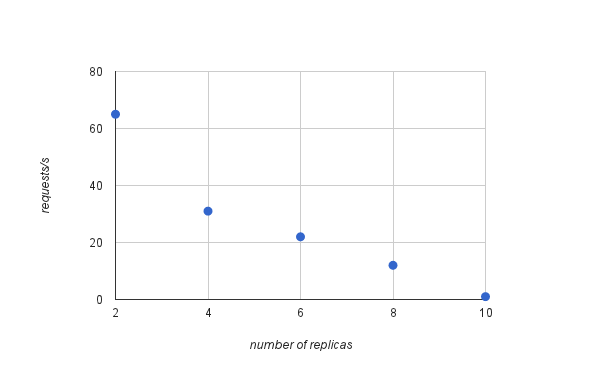
\includegraphics[scale=.50]{replicas.png}}
\caption{Performance of a one-group configuration rapidly deteriorates as the number of replicas increases}
\label{fig:replicas}
\end{figure}

\begin{figure}[H]
\centering
\makebox[\textwidth][c]{
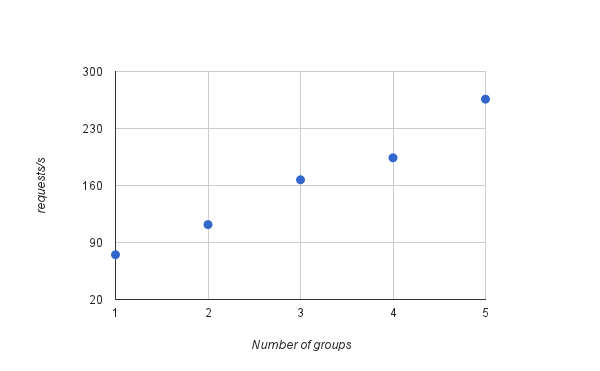
\includegraphics[scale=.5]{groups.png}}
\caption{Performance increases linearly as the number of groups increases. There is probably a saturation point, but we didn't have enough cluster machines to reach it.}
\label{fig:groups}
\end{figure}

\subsubsection{Paxos RPC Counts}

Multipaxos decreases the number of RPCs needed to reach agreement.

% Please add the following required packages to your document preamble:
% \usepackage[table,xcdraw]{xcolor}
% If you use beamer only pass ``xcolor=table'' option, i.e. \documentclass[xcolor=table]{beamer}
\begin{table}[H]
\centering
\makebox[\textwidth][c]{
\begin{tabular}{|l|l|l|}
\hline
\multicolumn{3}{|c|}{\cellcolor[HTML]{C0C0C0}\textbf{Paxos RPC Counts}}                  \\ \hline
                                 & \textbf{Single Proposer} & \textbf{Multiple Proposer} \\ \hline
\textbf{Normal Paxos}            & 30                       & 89            \\ \hline
\textbf{Paxos with Leaders}      & 20                       & 27                         \\ \hline
\textbf{Leaders and Pre-prepare} & 17                       & 20                         \\ \hline
\end{tabular}
}
\end{table}

\subsubsection{Disk Recovery}
Raw time to write 1GB to database, HDD:  21.470750409s

Raw time to write 1GB to database, SSD:  6.1470524260s

Recovery time of a 1GB database using our system: TBD

\subsection{Bottlenecks}
Although we made significant improvements performance-wise, we
identified a number of bottlenecks.

One notable bottleneck is disk writes. The database library we used,
levedb, uses a cache and is quite fast. However, in the process of
debugging networked RPCs, we implemented simple logging. This logging
slowed down the operations by nearly a factor of ten. This was a good
demonstration of how care must be taken in even the most mundane
aspects, such as logging.

Another bottleneck is network capacity and/or number of messages. As
shown in the latency and thoughput section, the increasing the number
of replicas has an adverse effect on performance since each operation
requires communication with a majority of replicas. 

Increasing the number of replica groups increases the performance of
the system for normal operation, especially under heavy load with
evenly distributed key requests. This is especially noticable in the
system throughput metric.  The number of groups roughly corresponds to
how parallelizable the operations are.

Using multipaxos reduces the amount of network communication required,
which improves the throughput and latency by about a factor of
two. Multipaxos also reduces the amount of paxos state information,
since prepares are pre-determined. This saves some disk space.  We
also suspect that using UDP would also improve throughput, as servers
that do not recieve a response already re-transmit their request,
making the TCP ack system redundant.

\section{Conclusion}
We did a project.

%{\footnotesize \bibliographystyle{acm}
%\bibliography{paper}}
%\newpage
\end{document}
